% ai-phishing-detection-dissertation/report/sections/4-results/xai-for-random-forest-using-shap/gloal-feature-importance.tex


\subsubsection*{Global feature importance}
Global feature importance through SHAP shows the importance TF-IDF features (terms or n-grams) that contributed the most to final classification of the Random Forest model. The below SHAP summary plot visualises these features, and they are ranked bu their sum of SHAP value magnitudes (Shapley values) across all samples. The plot showcases the SHAP values for each feature, indicating if a feature's value pushes the model's prediction to phishing (positive SHAP value) or away, i.e. ham (negative SHAP value). Feature values are denoted by their colour, with red meaning high feature value and blue meaning low feature value. Features are sorted by their mean absolute SHAP value, ranking their overall importance in the final classification.

\begin{figure}[H]
  \begin{center}
    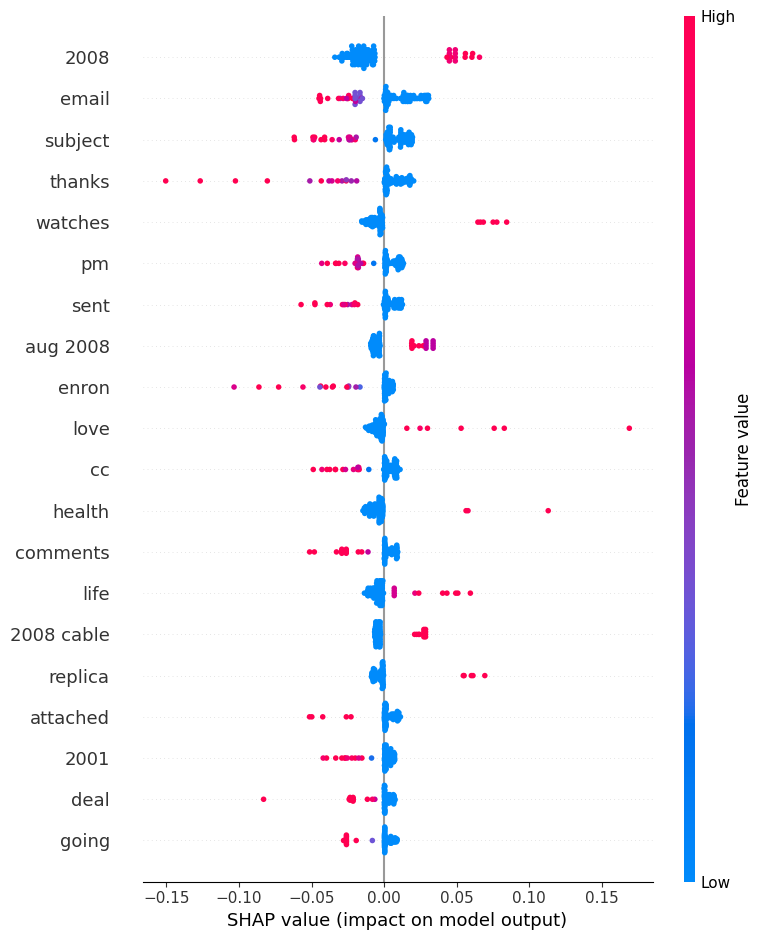
\includegraphics[scale=0.85]{xai-visualisations/random-forest/shap-global-feature-importance.png}
    \caption{SHAP summary plot for Random Forest global feature importance}
  \end{center}
\end{figure}

\noindent Based on the SHAP summary plot, certain top features clearly influenced the model's classification, with features like "thanks" and "enron" having a major negative impact influencing the model's prediction to the ham class, where as "watches" and "love" having a positive impact, pushing the model's prediction towards the phishing class.
